\documentclass[officiallayout]{tktla} 
%\documentclass[officiallayout,a4frame]{tktla}
\usepackage[latin1]{inputenc}
\usepackage{latexsym}
\usepackage{graphicx}
\usepackage{amsmath}
\usepackage{amssymb}
\usepackage{tikz}
\usetikzlibrary{arrows}
\usetikzlibrary{decorations.pathmorphing}
\usetikzlibrary{fit}					% fitting shapes to coordinates
\usetikzlibrary{backgrounds}
\tikzset{basic/.style={draw,fill=blue!50!green!20,
                       text badly centered,minimum width=3em}}
\tikzset{input/.style={basic,circle}}
\tikzset{weights/.style={basic,rectangle,minimum width=2em}}
\tikzset{functions/.style={basic,circle,fill=blue!50!green!20}}
\def\layersep{2.5cm}


\newcommand{\addsymbol}{\draw[thick] (0.5em,0.5em) -- (0,0.5em) -- 
                        (0,-0.5em) --  (-0.5em,-0.5em)
                        (0em,0.75em) -- (0em,-0.75em)
                        (0.75em,0em) -- (-0.75em,0em);}
                        
                        
\usepackage[]{algorithm2e}

% 
\usepackage{xargs}
\usepackage[colorinlistoftodos,prependcaption,textsize=tiny]{todonotes}
\newcommandx{\unsure}[2][1=]{\todo[linecolor=red,backgroundcolor=red!25,bordercolor=red,#1]{#2}}
\newcommandx{\change}[2][1=]{\todo[linecolor=blue,backgroundcolor=blue!25,bordercolor=blue,#1]{#2}}
\newcommandx{\info}[2][1=]{\todo[linecolor=OliveGreen,backgroundcolor=OliveGreen!25,bordercolor=OliveGreen,#1]{#2}}
\newcommandx{\improvement}[2][1=]{\todo[linecolor=red,backgroundcolor=red!25,bordercolor=red,#1]{#2}}
\newcommandx{\thiswillnotshow}[2][1=]{\todo[disable,#1]{#2}}
%


\title{Deep Learning Algorithms \\ for Control}
\author{Yuan Gao}
\authorcontact{gaoyuankidult@gmail.com\par
  http://www.cs.helsinki.fi/u/yuangao/}
\pubtime{September}{2015}
\reportno{0}
\isbnpaperback{000-00-0000-0}
\isbnpdf{000-00-0000-0}
\issn{1238-8645}
\printhouse{Unigrafia}
\pubpages{7} % --- remember to update this!
% For monographs, the number of the last page of the list of references
% For article-based theses, the number of the last page of the list of
% references of the preamble part + the total number of the pages of
% the original articles and interleaf pages.
\supervisorlist{Dorota Glowacka, University of Helsinki, Finland \newline  Leo K{\"a}rkk{\"a}inen, Nokia Research Center, Finland \newline Honkala Mikko Nokia Research Center, Finland}
\preexaminera{}
\preexaminerb{}
\opponent{}
\custos{}
\generalterms{}
\additionalkeywords{}
\crcshort{A.0, C.0.0}
\crclong{
\item[A.0] Example Category
\item[C.0.0] Another Example
}
\permissionnotice{
  To be presented in \ldots{} text of a long permission notice. Text of
  a long permission notice. Text of a long permission notice. Text of
  a long permission notice. Text of a long permission notice. Text of
  a long permission notice.
}

\newtheorem{theorem}{Theorem}[chapter]
\newenvironment{proof}{\noindent\textbf{Proof.} }{$\Box$}

\begin{document}

\frontmatter

\maketitle
\listoftodos
\begin{abstract}
Controlling a complicated mechanical system to perform a certain task, for example, making robot to dance, is a traditional problem studied in the area of control theory. Many successful applications like Google BigDog\cite{Raibert2008} and Google Self-driving car \todo{citation of self driving car} have been made in accordance to the new theories found in this field.

However more evidences show that in-cooperating with machine learning techniques in robotics can enable people to get rid of tedious engineering works of adjusting environmental parameters\todo{citation}. Many researchers like Jan Peters\todo{citation}, Sethu Vijayakumar, Stefan Schaal, Andrew Ng and Sebastian Thrun are the early explorers in this field. Based on the Partial Observable Markov Decision Process(POMDP) reinforcement learning, they contributed theory and practical implementation of several bench marks in this field.

Recently, one sub-field of machine learning called deep learning gained a lot of attention as a method attempting to model high-level abstractions by using model architectures composed by multiple non-linear layers. (for example \cite{Krizhevsky2012}). Several architectures of deep learning networks like deep belief network \cite{Hinton2006}, deep Boltzman machine \cite{Salakhutdinov2009}, convolutional neural network \cite{Krizhevsky2012} and deep de-noising auto-encoder \cite{Vincent2010} have shown its advantages in specific areas. Especially, convolutional neural network, which was invented by Krizhevsky, outperformed all the traditional feature-based machine learning techniques in ImageNet competition.

The main works of deep learning is more related to perception which deals with the problems like Sensor Fusion{OConnor2013}, Nature Language Processing(NLP)\cite{Cho2014} and Object Recognition\cite{Lenz2013}\cite{Hoffman2014}. Although considered briefly in J{\"u}rgen Schmidhuber's team\cite{Mayer2006}, the other area of robotics, namely control, remains more-or-less unexplored in the realm of deep learning.

There are two reasons about why these areas remain unexplored. The first reason is that deep learning method emphasizes on data driving techniques in which we need a lot of data to enable system to find important features whilst we don't have any dataset that can offer large amount of data. The second reason is that applying deep learning techniques requires introducing real robot platform to test the algorithm. This process is hard for researchers as they normally don't have resources for this complicated task.

The main focus of this thesis is to introduce general learning methods for robot control problem with an emphasize on deep learning method. As a consequence, this thesis tries to describe the transitional learning method as well as the emerging deep learning methods for robot control problem.

Ultimately, the author hope the readers of this thesis, even without much background in machine learning or robotics can understand the gists of solution for robot learning problems. \improvement{All paragraphs abstract needs to be rechecked.}
\end{abstract}

\begin{acknowledgements}
  This is a sample sentence that should look like normal text, and
  this is another. This is a sample sentence that should look like
  normal text, and this is another. This is a sample sentence that
  should look like normal text, and this is another.
\end{acknowledgements}

\tableofcontents

\mainmatter
\chapter{Introduction}

Controlling a complicated mechanical system to perform a certain task, for example making robot to dance, is a traditional problem studied in the field of control theory. Many successful applications like Google BigDog\cite{Raibert2008} and Google Self-driving car \cite{Guizzo2011a} have been made in accordance to the new theories found in this field.

However more evidences show that in-cooperating with machine learning techniques in robotics can enable people to get rid of tedious engineering works of adjusting environmental parameters\todo{citation}. Many researchers like Jan Peters\todo{citation}, Sethu Vijayakumar, Stefan Schaal, Andrew Ng and Sebastian Thrun are the early explorers in this field. Based on the Partial Observable Markov Decision Process(POMDP) reinforcement learning, they contributed first several algorithms enabling robot to learn to perform a certain task overtime.

Recently, one sub-field of machine learning called deep learning gained a lot of attention as a method attempting to model high-level abstractions by using model architectures composed by multiple non-linear layers. (for example \cite{Krizhevsky2012}). Several architectures of deep learning networks like deep belief network \cite{Hinton2006}, deep Boltzman machine \cite{Salakhutdinov2009}, convolutional neural network \cite{Krizhevsky2012} and deep de-noising auto-encoder \cite{Vincent2010} have shown its advantages in specific areas. Especially, convolutional neural network, which was invented by Krizhevsky, outperformed all the traditional feature-based machine learning techniques in ImageNet competition.

Based on the two trends we noticed, a natural path of research is to use deep learning methods for controlling movements of robot. Until the end of 2014,  the main works of deep learning are more related to a category of robotics called perception, which deals with problems like Sensor Fusion \cite{OConnor2013}, Nature Language Processing(NLP)\cite{Cho2014} and Object Recognition\cite{Lenz2013}\cite{Hoffman2014}. Although considered briefly in J{\"u}rgen Schmidhuber's team\cite{Mayer2006}, the other area of robotics, namely control, remains more-or-less unexplored in the realm of deep learning.

The researches done in J{\"u}rgen Schmidhuber's team provided several interesting structures that might be potentially useful for robot control. The name of one of these structures is called Long Short Term Memory (LSTM), which is one variation of Recurrent Neural Network(RNN). Several experiments like generating sequences\cite{Graves2013}, speech recognition\cite{Graves2013b} and neural turing machine \cite{Graves2014} show that it has ability of extracting and storing temporal information from data. As a consequence, this specific structure of RNN, with modification, can be applied for control problems of robots.

There are two main focuses of this thesis. One main focus of this Thesis is to introduce general learning methods for robot control problem with an emphasize on deep learning method. this thesis tries to describe the transitional learning method as well as the emerging deep learning methods for robot control problem. Anther focus of this thesis is to introduce the main contribution of author in this field. With experiments, the author is able to show his own method can outperform the transitional machine learning methods of robot control problems.

\chapter{Reinforcement Learning}

If we would like to discuss what might be the most common way of learning, learning based on interacting with our environment is a natural idea to think about. When we were born in this world, we had no teachers around us. But tens of years passed, we learned to fear, to communicate with others and to write a paper. As a consequence, it is very natural to think that our environment is a great source of information. While playing around with environment, we learn by taking actions and getting reward from it. Now when we cook , when we do exercise, we are fully and acutely aware what will be the response of environment.

The RL is an area that studies the mechanism of the such kind of learning in a computational way. Generally the goal of RL is to find a way of mapping different states with different actions so that we could maximize the reward signals. 

There are two main approaches in area of reinforcement learning, one is based on Markov Decision Process(MDP)\cite{Sutton1998a}. Both methods have advantages and drawbacks when applied to robotics, another one is recurrent neural network(RNN)\cite{williams1989learning}.

In the following sections of this chapter, we may consider robot as an agent in all description of related techniques.

\section{Markov Decision Process}
Markov Decision Process (MDP) is a discrete time stochastic control process. We may consider a robot in a state $s$ of discrete state space $S$. The robot can take an action $a$ in all possible action set $A$ resulting in a state $s'$ . We can denote this process as transition function
$P_a(s, s')$ meaning the probability of moving from state
$s$ to state $s'$ through action a. Then after the robot executes action $a$ and results in $s'$ , it will receive a reward $r$ according to reward function denoted as $R_a(s, s ')$. The goal of reinforcement learning is to optimize cumulative reward of whole process. 

The problems of MDP is more clear to researchers as it is based on mathematical formalizations. On one hand, MDP-based methods together with optimization methods such as Gradient Partially Observable Markov Decision Processes (GPOMDP), projection method or nature gradient are state-of-art in robot trajectory learning. On another hand, as data collected from robot is different from normal data, it was pointed out the MDP-based methods suffers several curses\cite{Kober2013}.
\begin{itemize}
\item Curse of Dimensionality
\item Curse of Real-World Samples
\item Curse of Under-Modeling and Model Uncertainty
\item Curse of Goal Specification
\end{itemize}
The data is normally high dimensional, continuous and erroneous data in robot systems. It is considered to be difficult questions to neglect these issues and it is also hard to specify the goal of system i.e. what robot needs to be at last.

\subsection{Partially Observable Markov Decision Process}
A partially observable Markov decision process (POMDP) is a generalization of a Markov decision process (MDP). A POMDP models an agent decision process in which it is assumed that the system dynamics are determined by an MDP, but the agent cannot directly observe the underlying state. Instead, it must maintain a probability distribution over the set of possible states, based on a set of observations and observation probabilities, and the underlying MDP.

The POMDP framework is general enough to model a variety of real-world sequential decision processes. Applications include robot navigation problems, machine maintenance, and planning under uncertainty in general. The framework originated in the operations research community, and was later taken over by the artificial intelligence and automated planning communities.

An exact solution to a POMDP yields the optimal action for each possible belief over the world states. The optimal action maximizes (or minimizes) the expected reward (or cost) of the agent over a possibly infinite horizon. The sequence of optimal actions is known as the optimal policy of the agent for interacting with its environment.
\todo{This introduction needs to be changed latter}

More precisely, the POMDP is a discrete time stochastic control process. We may consider a robot in a state $s_t$ of discrete space $\mathcal{S}$ where t means iteration number. Now the robot can take an action a in all possible action set A resulting in a state $s_{t+1}$. We can denote this process as transition function Ta($s_t$,$s_{t+1}$) meaning the probability of moving from state $s_t$ to state $s_{t+1}$ through action $a$. Then after the robot executes action a and results in st+1, it will receive a reward according to reward function denoted as $R_a(s_t,s_{t+1}$).

Formally, we define MDP as follows:

A Markov decision process is a 4-tuple denoted as ($S$,$A$,$T\cdot(\cdot,\cdot)$,$R\cdot(\cdot,\cdot)$)
In this tuple
\begin{itemize}
\item	$\mathcal{S}$ is a finite set of states. It describes all possible states of the space.
\item	$\mathcal{A}$ is a finite set of actions. It describes all possible states that robot can take.
\item	$T\cdot(\cdot,\cdot)$ is a function that takes three arguments. e.g $T_{a_t}(s_t,s_{t+1})$ means probability of transferring from $s_t$ to $s_{t+1}$ with action $a_t$.
\item	$R\cdot(\cdot,\cdot)$ is also a function that takes three arguments. e.g $R_{a_t}(s_t,s_{t+1})$ means reward of transferring from $s_t$ to $s_{t+1}$ with action $a_t$.
\end{itemize}


The main problem of reinforcement learning is to find a policy function $\pi(s) : s \rightarrow a$ to map every state s with action $a$ so that a cumulative reward $R$ is maximized, where $0 \leq \gamma \leq 1$ is a discount factor. As the discount factor generalizes discounted situation and undiscounted situation, it broadens our theory.

\subsection{Markov Decision Process with Continuous States}
Now considering the environment of robots, we need some modifications to original POMDP. First we still assume the process to be discrete time but we consider continuous space $S \in R^n$ and continuous action set $A \in R^m$ where $n$ is dimension of space and $m$ is dimension of actions. For initial state $s_0$, we assign a distribution $p(s_0)$ where $s_0 \in \mathcal{S}$. At any state $s_t \in \mathcal{S}$, we have a continuous policy $\pi(a_t|s_t) = p(a_t|s_t,\theta)$ parametrized by $\theta$. Transfer function now also becomes continuous. It is corresponded to a probability distribution $T_{a_t}(s_t,s_{t+1}) = p(s_{t+1}|s_t,a_t)$. After this step is completed, the process will general a reward function $R_{a_t}(s_t,s_{t+1}$) which is defined as $R\cdot(\cdot,\cdot) : S  \times S \times A \rightarrow [0,\inf)$.
After these modifications, we can now formalize continuous MDP.

Continuous Markov Decision Process With Infinite States is a modified version of ordinary POMDP. Mathematically, it is defined as a 5-tuple ($P_{init},S,A,T\cdot(\cdot,\cdot),R\cdot(\cdot,\cdot))$ where in this tuple
\begin{itemize}
\item	$P_{init}$ is a initial distribution of the states.
\item	$S = Rn$ is a infinite set of states. It describes all possible states of the space.
\item	$A = Rm$ is a infinite set of actions. It describes all possible actions of the agent.
\item	$T\cdot(\cdot,\cdot)$ is a function that takes three arguments. e.g $Tat(st,st+1)$ means probability of transferring from st to st+1 with action at.
\item	$R\cdot(\cdot,\cdot)$ is a function that takes three arguments. e.g $Rat(st,st+1)$ means reward of transferring from st to st+1 with action at.
\end{itemize}

With this continuous setting, we have objective function defined as follows:
\begin{figure}[h!]

  \centering
    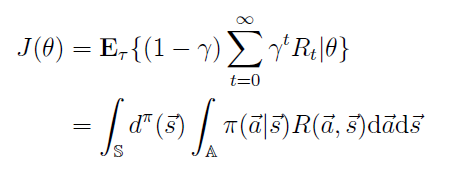
\includegraphics[width=0.5\textwidth]{objective_func}
\end{figure}

Where $d^\pi(\vec{s})$ refers to $1 - \gamma^tp(\vec{s} = \vec{s_t})$, $0 \geq \gamma \geq 1$ refers to discount factor and $\pi(\vec{a}|\vec{s})$ is parametrized by $\theta$.
\subsection{Value Functions}
We define two functions to further describes this process. First function is statevalue
function denoted as $V^\pi(\vec{x})$. This means expected value of an agent that follows
an policy of $\pi$ with initial value $\vec{s}$. It characterizes the rewards of following a policy $\pi$. Mathematically, it is defined as:

\begin{figure}[h!]
  \centering
    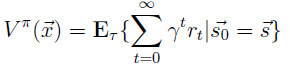
\includegraphics[width=0.4\textwidth]{value1}
\end{figure}
where $\tau$ stands for trajectory of agent.
\begin{figure}[h!]
  \centering
    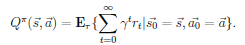
\includegraphics[width=0.5\textwidth]{value2}
\end{figure}
State-value function only depends on the first state of agent. After that the system
is governed by policy $\pi$. Another value function we need to defines is state-action
value function.
\subsection{Natural Actor Critic Model}
The first thing of demonstrating Natural Actor-Critic is to explain the term. Natural
stands for gradient framework called natural gradient while Actor-Critic means an
iterative method of evaluating and improving objective function.

Robot learning is based on Markov Decision Process with discrete time and continuous
states. The objective function is defined in section Markov Decision Process
by Formula 1. A normal gradient of objective function is defined as :


\begin{figure}[h!]
  \centering
    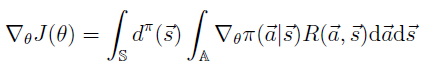
\includegraphics[width=0.5\textwidth]{actor_critic}
\end{figure}

Please note $\theta$ is related to $\pi(\vec{a}|\vec{s})$ as it is defined by $\pi(\vec{a}|\vec{s}|\theta)$.

However, here we need to redefine this gradient as vanilla gradient. Pointed out
and nicely presented by Shun-ichi Amari, another kind of gradient called natural
gradient is more efficient in many machine learning application than vanilla gradient.
Mathematically we define following formula as natural gradient:
\begin{equation}
\nabla J(\theta) = G^{-1}\nabla J(\theta)
\end{equation}

Where G is fisher information metrix[].
Fisher information matrix is a matrix defined on Romanian space. This metric
is interesting on several aspects. One of them is that it shows true direction of
a function's steepest direction and on the contrary, the vanilla gradient does not.
The long proof of previous statement is based by showing natural gradient descent
method is fisher efficient. We recommend a further reading on Amari's paper[].

If we rewrite Formula 5 as:

\begin{figure}[h!]
  \centering
    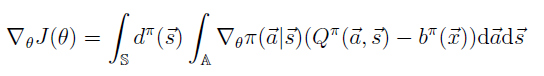
\includegraphics[width=0.7\textwidth]{gradient}
\end{figure}

Where $Q^\pi(a, s)$ is state-action value function and $b^\pi(x)$ is kind of baseline. Two
papers [] [] demonstrate why $R(s, a)$ is replace by $Q^\pi(a, s) - b^\pi(x)$. It can be
shown that $R(s, a)$ is further approximated as $(\nabla_\theta \log\pi(a,s)^\pi(s))^T \vec{w}$ parametrized by $\vec{w}$.
\section{Reinforcement Learning Methods}
\subsection{Temporal Difference Learning}
\subsection{Q-Learning}
\subsection{Adaptive Heuristic Critic}
\subsection{Prioritised Sweeping}
\subsection{Policy Gradient Methods}

\section{Classification of the Regarded RL Problems}
\subsection{High-Dimensionality}
\subsection{Partial-Observability}
\subsection{Continuous State and Action Spaces}
\subsection{Data-Efficiency}

\chapter{Recurrent Neural Networks}
Recurrent Neural Network(RNN) is a special structure of neural network that has recurrent connections. In the following sections of this chapter, we are going to discuss the details of this model.
\section{Feedforward Neural Networks}
In year 1957, the simplest structure of neural network called perceptron was introduced by Frank Rosenblatt in Conell's Aeronautical Laboratory. This model consists only one cell and multiple connections. Figure~\ref{perceptron} shows the basic structure of perceptron.
\begin{figure}[h!]
  \centering
	\begin{tikzpicture}[scale=1.2, shorten >=1pt,->,draw=black!80, node distance=\layersep]
    \tikzstyle{every pin edge}=[<-,shorten <=1pt]
    \tikzstyle{neuron}=[circle,fill=black!25,minimum size=17pt,inner sep=0pt]
    \tikzstyle{annot} = [text width=4em, text centered]
            
    
    \node[neuron] (sum) at (4,0) {$\sum$};
    \foreach \h [count=\hi ] in {$x_n$,$x_2$,$x_1$,$1$}{%
          \node[neuron] (f\hi) at (2,\hi*1cm-2.5 cm) {\h};
          \draw[->] (f\hi) -- (sum);
		}

    \node[neuron] (tanh) at (6,0) {};
       \begin{scope}[xshift=6cm,scale=.75]
         \node [] {$tanh$};
       \end{scope}
    \draw[->] (sum) -- (tanh);
    \draw[->] (tanh) -- ++(1,0);
    % Labels
    \node[above=1cm]  at (f4) {inputs};
    \end{tikzpicture}
  \caption{This picture shows the structure of perceptron, the i'th input is shown as $x_i$ and corresponded weights are denoted as $w_i$. There is also a bias term name $b$ connected to cell, which, with a addition function, generates the output.}\label{proceptron}
\end{figure}

The formula of representing input and output is defined as:

\begin{equation}
y = \mathbf{w}\cdot\mathbf{x} + b
\end{equation}

If we consider $b$ also as one of the inputs, then the formula can be defined as:

\begin{equation}
y = \hat{\mathbf{w}}\hat{\cdot\mathbf{x}}
\end{equation}\label{pronceptron_formula}

where $ \hat{\mathbf{w}} = [\mathbf{w};b] $ and $\hat{\mathbf{x}} = [\mathbf{x};1]$.

This simple structure was considered promising initially from several points of view. But after further investigation, the perceptron was proven that it can not classify many non-linear classes of patterns. However, its discovery leads to a field of research called neural networks in area artificial intelligence. As a consequence, since 1957, people started trying different methods for modifying this model to adapt to different problems. One important modification is to add a non-linear transformation function to the system i.e. after getting $y$ from Formula\ref{pernceptron_formula}, we use a function like tanh to get a new $\hat{y}$ to ensure the output is restricted in a range. Anther important modification of the system is to stack many perceptrons together to build a large and complex model for the classification purpose. This kind of networks is normally called Feed-forward Neural Networks(FFNN) as information send to this system is propagated only from lower layer to higher layer. Figure~\ref{feedforward_nn} shows the structure of FFNN system.



\begin{figure}[h!]
  \centering

	\begin{tikzpicture}[scale=1.2, shorten >=1pt,->,draw=black!80, node distance=\layersep]
    \tikzstyle{every pin edge}=[<-,shorten <=1pt]
    \tikzstyle{neuron}=[circle,fill=black!25,minimum size=17pt,inner sep=0pt]
    \tikzstyle{annot} = [text width=4em, text centered]

    % Draw the input layer nodes
    \foreach \name / \y in {1/1,2/2,$d$/4}
    % This is the same as writing \foreach \name / \y in {1/1,2/2,3/3,4/4}
        \node[neuron] (I-\name) at (0,-\y) {\name};
    \node (I-3) at (0,-3) {\vdots};

    % Draw the hidden layer nodes
    \foreach \name / \y in {1/1,2/2,$K$/5}
        \path[yshift=0.5cm]
            node[neuron] (H-\name) at (\layersep,-\y cm) {\name};
    \node (H-3) at (\layersep,-3) {\vdots};

    \foreach \name / \y in {1/1.5,2/2.5,$M$/4.5}
        \path[yshift=0.5cm]
            node[neuron] (O-\name) at (2*\layersep,-\y cm) {\name};
    \node (O-3) at (2*\layersep,-3) {\vdots};

    % Connect every node in the input layer with every node in the
    % hidden layer.
    \foreach \source in {1,2,$d$}
        \foreach \dest in {1,2,$K$}
            \path (I-\source) edge (H-\dest);
    
   
    % Connect every node in the hidden layer with the output layer
    \foreach \source in {1,2,$K$}
        \foreach \dest in {1,2,$M$}
            \path (H-\source) edge (O-\dest);

    % Annotate the layers
    \node[annot,above of=H-1, node distance=1cm] (hl) {Hidden layer};
    \node[annot,left of=hl] {Input layer};
    \node[annot,right of=hl] {Output layer};
	\end{tikzpicture}
  \caption{This picture shows the structure of Feed-forward Neural Network. There are three layers in this network, namely the input layer, hidden layer and the output layer. For connections from input layer to hidden layer, the i'th input is shown as $x_i$ and corresponded weights of hidden neuron $j$ is denoted as $W_{ij}$.}\label{feedforward_nn}
\end{figure}

The formula describing the each layer is then defined as:

\begin{equation}
\mathbf{o} = \sigma(W\mathbf{x})
\end{equation}
where $f(\cdot)$ is a non-linear transformation function.(e.g. tanh)

\section{Recurrent Neural Networks}
The Recurrent Neural Networks(RNN) contain at least one neuron that has at least one recurrent connection i.e. a connection that connects to itself or to lower layer. This special structure makes memory cell to be internal memory which enables network to memories the change of sequential data. Unlike the feed-forward neural network, the recurrent neural network is used for predicting next data point.

\begin{figure}[h!]
  \centering
  \begin{tikzpicture}[scale=1.2, shorten >=1pt,->,draw=black!80, node distance=\layersep]
    \tikzstyle{every pin edge}=[<-,shorten <=1pt]
    \tikzstyle{neuron}=[circle,fill=black!25,minimum size=17pt,inner sep=0pt]
    \tikzstyle{annot} = [text width=4em, text centered]

    % Draw the input layer nodes
    \foreach \name / \y in {1/1,2/2,$d$/4}
    % This is the same as writing \foreach \name / \y in {1/1,2/2,3/3,4/4}
        \node[neuron] (I-\name) at (0,-\y) {\name};
    \node (I-3) at (0,-3) {\vdots};

    % Draw the hidden layer nodes
    \foreach \name / \y in {1/1,2/2,$K$/5}
        \path[yshift=0.5cm]
            node[neuron] (H-\name) at (\layersep,-\y cm) {\name};

    \node (H-3) at (\layersep,-3) {\vdots};

    \foreach \name / \y in {1/1.5,2/2.5,$M$/4.5}
        \path[yshift=0.5cm]
            node[neuron] (O-\name) at (2*\layersep,-\y cm) {\name};
    \node (O-3) at (2*\layersep,-3) {\vdots};

    % Connect every node in the input layer with every node in the
    % hidden layer.
    \foreach \source in {1,2,$d$}
        \foreach \dest in {1,2,$K$}
            \path (I-\source) edge (H-\dest);
    
    % Connect hidden layer to hidden layer
    \foreach \source in {1,2,$K$}
		\path (H-\source) edge [loop above] (H-\source);
    
    
    % Connect every node in the hidden layer with the output layer
    \foreach \source in {1,2,$K$}
        \foreach \dest in {1,2,$M$}
            \path (H-\source) edge (O-\dest);
\end{tikzpicture}
  \caption{This picture shows the structure of recurrent neural network. There are two layers in this networ namely input layer and hidden layer, the first layer contains notes connected to the input data. The second layer stores information and also forwards information to next layer. The cell in the hidden layer has a connection to itself which means the information stored in the cell at time $t-1$ also influences the information stored in the cell at time $t$}\label{feedforward_nn}
\end{figure}

\subsection{Finite Unfolding in Time}
When considering the structure of neural network, people normally application Finite Unfolding in Time for RNN. It means to introduce another dimension for RNN. In this way, the recurrent connection can be dealt with more easily.  In the following section, we will use a simple example for explaining this idea. The model we are going to use contains one input neuron, one hidden neuron and one output neuron. See Figure~\ref{simple_rnn} for reference.
\begin{figure}[h!]
  \centering

  \caption{This picture shows the structure of a simple RNN. It contains three layers i.e. one input layer, one hidden layer and one output layer.}\label{simple_rnn}
\end{figure}
\change{This picture should be remade using tikz later}

In this figure, we mark input layer as $\mathbf{x}$, hidden layer as $\mathbf{s}$ and output layer as $\mathbf{o}$.

The basics idea of unfolding RNN in time is to copy RNN several times and connect them in a chronological order. If the connection is recurrent, then the connection should be connect to the same neuron of next time step.Figure~\ref{unfolded_simple_rnn} illustrates the model of unfolding simple RNN  for three time steps.

\begin{figure}[h!]
  \centering
% The input, state transition, and measurement matrices
% are represented by gray squares.
% They have a smaller minimal size for aesthetic reasons.
\tikzstyle{matrx}=[rectangle,
                                    thick,
                                    minimum size=1cm,
                                    draw=gray!80,
                                    fill=gray!20]


% Everything is drawn on underlying gray rectangles with
% rounded corners.
\tikzstyle{background}=[rectangle,
                                                fill=gray!10,
                                                inner sep=0.5cm,
                                                rounded corners=5mm]

\begin{tikzpicture}[>=latex,text height=1.5ex,text depth=0.25ex]
    % "text height" and "text depth" are required to vertically
    % align the labels with and without indices.
  
  % The various elements are conveniently placed using a matrix:
  \matrix[row sep=0.5cm,column sep=0.5cm] {
    % First line: Control input
    		&
        \node (x_t-1) [matrx]{$\mathbf{x}_{t-1}$}; &
        &
        \node (x_t)   [matrx]{$\mathbf{x}_t$};     &
        &
        \node (x_t+1) [matrx]{$\mathbf{x}_{t+1}$}; &

        \\
        % Third line: State & state transition matrix
		\\
		&
        \node (s_t-1) [matrx] {$\mathbf{s}_{t-1}$}; &
		&
        \node (s_t)   [matrx] {$\mathbf{s}_t$};     &
		&
        \node (s_t+1) [matrx] {$\mathbf{s}_{t+1}$}; &
		\\
		\\

        % Fifth line: Measurement
        &
        \node (o_t-1) [matrx] {$\mathbf{o}_{t-1}$}; &
        &
        \node (o_t)   [matrx] {$\mathbf{o}_t$};     &
        &
        \node (o_t+1) [matrx] {$\mathbf{o}_{t+1}$}; &
        \\
    };
    
    % The diagram elements are now connected through arrows:
    \path[->]
    	    (x_t-1) edge[thick] (s_t-1)
        (x_t) edge[thick] (s_t)
        (x_t+1) edge[thick] (s_t+1)
        	        	
        (s_t-1) edge[thick] (s_t)
        (s_t) edge[thick] (s_t+1)  
        
    	    (s_t-1) edge[thick] (o_t-1)
        (s_t) edge[thick] (o_t)
        (s_t+1) edge[thick] (o_t+1)
        ;
    
    % Now that the diagram has been drawn, background rectangles
    % can be fitted to its elements. This requires the TikZ
    % libraries "fit" and "background".
    % Control input and measurement are labeled. These labels have
    % not been translated to English as "Measurement" instead of
    % "Messung" would not look good due to it being too long a word.
    \begin{pgfonlayer}{background}
        \node [background,
                    fit=(x_t-1) (x_t+1),
                    label=left:Inputs:] {};
        \node [background,
                    fit=(s_t-1) (s_t+1),
                    label=left:Hidden States:] {};
        \node [background,
                    fit=(o_t-1) (o_t+1),
                    label=left:Outputs:] {};
    \end{pgfonlayer}
\end{tikzpicture}
  \caption{This picture contains model that unfolds a simple RNN described in Figure\ref{simple_rnn} in three time steps. In this figure, $x_t$ represents input layer at time $t$, $s_t$ representes the hiddent states at time $t$ and $o_t$ representes output layer at time $t$.}\label{unfolded_simple_rnn}
\end{figure}
\change{This picture should be remade using tikz later}

The finite unfolding technique transforms a neural network with recurrent connection to a network that is easier to compute gradients. It is also easy for us to write this neural network's expression.

\begin{equation}
\mathbf{s_{t}} = \sigma(W\mathbf{x_t} + B\mathbf{s_{t-1}})\label{internal_state_fomula}
\end{equation}
Where $\mathbf{s_t}$ is the value of hidden state at time $t$ and $B$ is the weight matrix for updating hidden state information from time $t-1$ to $t$.


\subsection{Overshooting}
Considering that we only one time series, the task for RNN is to predict next data point based on previous data we have. There are two steps for solving this problem. First we need to copy the data into two set and shift the input by one to produce output. It is illustrated as shown in Figure~\ref{overshot_rnn}.

\begin{figure}[h!]
  \centering
\tikzstyle{matrx}=[rectangle,
                                    thick,
                                    minimum size=1cm,
                                    draw=gray!80,
                                    fill=gray!20]


% Everything is drawn on underlying gray rectangles with
% rounded corners.
\tikzstyle{background}=[rectangle,
                                                fill=gray!10,
                                                inner sep=0.5cm,
                                                rounded corners=5mm]
\begin{tikzpicture}[>=latex,text height=1.5ex,text depth=0.25ex]
    % "text height" and "text depth" are required to vertically
    % align the labels with and without indices.
  
  % The various elements are conveniently placed using a matrix:
  \matrix[row sep=0.5cm,column sep=0.5cm] {
    % First line: Control input
		\node (x_t-2) [matrx]{$\mathbf{x}_{t-2}$}; &
    		&
        \node (x_t-1) [matrx]{$\mathbf{x}_{t-1}$}; &
        &
        \node (x_t)   [matrx]{$\mathbf{x}_t$};     &
        &
        & &

        \\
        % Third line: State & state transition matrix
		\\
		\node (s_t-2) [matrx]{$\mathbf{s}_{t-2}$}; &
		&
        \node (s_t-1) [matrx] {$\mathbf{s}_{t-1}$}; &
		&
        \node (s_t)   [matrx] {$\mathbf{s}_t$};     &
		&
        \node (s_t+1) [matrx] {$\mathbf{s}_{t+1}$}; &
		\\
		\\
		
        \node (hat_x_t-1) [matrx]{$\mathbf{\hat{x}}_{t-1}$}; &
        &
        \node (hat_x_t) [matrx] {$\mathbf{\hat{x}}_{t}$}; &
        &
        \node (hat_x_t+1)   [matrx] {$\mathbf{\hat{x}}_{t+1}$};     &
        &
        \node (hat_x_t+2) [matrx] {$\mathbf{\hat{x}}_{t+2}$}; &
        \\
    };
    
    % The diagram elements are now connected through arrows:
    \path[->]
    		(x_t-2) edge[thick] (s_t-2)
    	    (x_t-1) edge[thick] (s_t-1)
        (x_t) edge[thick] (s_t)
        	  
	    (s_t-2) edge[thick] (s_t-1)        	        	
        (s_t-1) edge[thick] (s_t)
        (s_t) edge[thick] (s_t+1)  

		(s_t-2) edge[thick] (hat_x_t-1)       
    	    (s_t-1) edge[thick] (hat_x_t)
        (s_t) edge[thick] (hat_x_t+1)
        (s_t+1) edge[thick] (hat_x_t+2)
        ;
    
    % Now that the diagram has been drawn, background rectangles
    % can be fitted to its elements. This requires the TikZ
    % libraries "fit" and "background".
    % Control input and measurement are labeled. These labels have
    % not been translated to English as "Measurement" instead of
    % "Messung" would not look good due to it being too long a word.

\end{tikzpicture}
  \caption{This figure isllustrates in a predictive model made by RNN, how does it generate $\hat{x_t}$ based on previous data. After using all training example, the model lacks input data. Then the neural caluclation of hidden defined as $\mathbf{s_{t}} = \sigma(W\mathbf{x_t} + B\mathbf{s_{t-1}}))$ becomes $\mathbf{s_{t}} = \sigma(B\mathbf{s_{t-1}})$}\label{overshot_rnn}
\end{figure}

Last training step takes input $\mathbf{x}(t-2)$, $\mathbf{x}(t-1)$, $\mathbf{x}(t)$ as input and produce $\mathbf{x}(t-1)$, $\mathbf{x}(t)$, $\mathbf{x}(t+1)$ as outputs. However it is very difficult to predict value at time t+2 as we don't have information of $\mathbf{x}(t+1)$. According to the Fomula~\ref{internal_state_fomula}, the input is set to $\mathbf{0}\quad \forall t > T$ then we get:

\begin{equation}
\mathbf{s_{t}} = \sigma(B\mathbf{s_{t-1}})\label{overshot_formula}
\end{equation}

As a consequence, the output defined as $\mathbf{x_{t+1}} = A\mathbf{s_{t}}$ becomes the prediction for next value. This phenomenon is called overshooting.
\subsection{Dynamical Consistency}

Dynamical consistency is kept by introducing the output of last time step to input of current time step. Figure~\ref{series_prediction_rnn} illustrates how is it done through the modification of structure.

\begin{figure}[h!]
  \centering
  \tikzstyle{matrx}=[rectangle,
                                    thick,
                                    minimum size=1cm,
                                    draw=gray!80,
                                    fill=gray!20]

\tikzstyle{dashed_matrx}=[rectangle,
                                    thick,
                                    dashed,
                                    minimum size=1cm,
                                    draw=gray!80,
                                    fill=gray!20]

\tikzstyle{background}=[rectangle,
                                                fill=gray!10,
                                                inner sep=0.5cm,
                                                rounded corners=5mm]
\begin{tikzpicture}[>=latex,text height=1.5ex,text depth=0.25ex]
    % "text height" and "text depth" are required to vertically
    % align the labels with and without indices.
  
  % The various elements are conveniently placed using a matrix:
  \matrix[row sep=0.5cm,column sep=0.5cm] {
    % First line: Control input
		\node (x_t-2) [matrx]{$\mathbf{x}_{t-2}$}; &
    		&
        \node (x_t-1) [matrx]{$\mathbf{x}_{t-1}$}; &
        &
        \node (x_t)   [matrx]{$\mathbf{x}_t$};     &
        &
        \node (x_t+1)   [dashed_matrx]{$\mathbf{\hat{x}}_{t+1}$}; 	  & 
        &

        \\
        % Third line: State & state transition matrix
		\\
		\node (s_t-2) [matrx]{$\mathbf{s}_{t-2}$}; &
		&
        \node (s_t-1) [matrx] {$\mathbf{s}_{t-1}$}; &
		&
        \node (s_t)   [matrx] {$\mathbf{s}_t$};     &
		&
        \node (s_t+1) [matrx] {$\mathbf{s}_{t+1}$}; &
		\\
		\\
		
        \node (hat_x_t-1) [matrx]{$\mathbf{\hat{x}}_{t-1}$}; &
        &
        \node (hat_x_t) [matrx] {$\mathbf{\hat{x}}_{t}$}; &
        &
        \node (hat_x_t+1)   [matrx] {$\mathbf{\hat{x}}_{t+1}$};     &
        &
        \node (hat_x_t+2) [matrx] {$\mathbf{\hat{x}}_{t+2}$}; &
        \\
    };
    
    % The diagram elements are now connected through arrows:
    \path[->]
    		(x_t-2) edge[thick] (s_t-2)
    	    (x_t-1) edge[thick] (s_t-1)
        (x_t) edge[thick] (s_t)
        (x_t+1) edge[thick,dashed] (s_t+1)
        	  
	    (s_t-2) edge[thick] (s_t-1)        	        	
        (s_t-1) edge[thick] (s_t)
        (s_t) edge[thick] (s_t+1)  

		(s_t-2) edge[thick] (hat_x_t-1)       
    	    (s_t-1) edge[thick] (hat_x_t)
        (s_t) edge[thick] (hat_x_t+1)
        (s_t+1) edge[thick] (hat_x_t+2)
        (hat_x_t+1) edge[thick, dashed, -latex, out=45,in=225] (x_t+1)
        ;
    
    % Now that the diagram has been drawn, background rectangles
    % can be fitted to its elements. This requires the TikZ
    % libraries "fit" and "background".
    % Control input and measurement are labeled. These labels have
    % not been translated to English as "Measurement" instead of
    % "Messung" would not look good due to it being too long a word.

\end{tikzpicture}
  \caption{This picture contains model for predicting data for time series. For the first unfolded structure of neural network, the data of series at time t-2 is fed to the network and we expect data at time t-1 are predict by the network.}\label{series_prediction_rnn}
\end{figure}

By remembering all the parameters in the network and unfold in time for several steps, the recurrent neural network is able to predict the next data point in the sequence. The relationship between input and output is listed as follows:

\begin{align}
\mathbf{s_{t}} &= \sigma(W\mathbf{x_t} + B\mathbf{s_{t-1}}) \\
\mathbf{x_{t+1}} &= A\mathbf{s_{t}}
\end{align}

where $A$ means weight matrix of internal states to output states.


To sum up, the dynamics of system becomes as follows.

\begin{align}
\mathbf{s_{t}} &= \sigma(W\mathbf{x_t} + B\mathbf{s_{t-1}}) \quad \forall x \leq T \label{training_rnn}\\ 
\mathbf{s_{t}} &= \sigma(W\mathbf{\hat{x}_t} + B\mathbf{s_{t-1}}) \quad \forall x > T \label{prediction_rnn}\\
\mathbf{o_{t+1}} &= A\mathbf{s_{t}} \quad \forall x \leq T - 1 \label{train_output}\\
\mathbf{\hat{x}_{t+1}} &= A\mathbf{s_{t}}  \quad \forall x > T - 1  \label{train_prediction}
\end{align}

Formula~\ref{training_rnn} shows how are values of internal states updated at the training stage. Formula~\ref{prediction_rnn} shows how are values of output data predicted after training stage. Formula~\ref{train_output} shows how outputs generated after training stage. Formula~\ref{train_prediction} shows how outputs predicted after training stage. The overall goal of the system is to minimize the different between the output and predicted output for all time series. Mathematically, it is defined as:

\begin{equation}
J = \sum_{i=1}^{T}\mathbf{o}_{t} - \mathbf{y}_{t}
\end{equation}

If we assume each input and output has N data points, then the cost becomes:

\begin{equation}
J = \sum_{i=1}^{T}\sum_{n=1}^{N}o^n_{t} - y^n_{t}
\end{equation}

The main goal of function is to minimize the cost over function parameters defined in the network.(See section ~\ref{training_rnn} for more reference.)

\section{Universal Approximation}
It has been proven that multi-layer feed-forward neural networks are universal approximators by Hornik in 1989. Similar works have also been mentioned by Cybenko and Funahashi in the same year. In this work, Hornik continued work of Minskey and Papert about two layers network. Minkey and Papert proved that two-layer neural networks are not able to approximate functions that do not belong to a special class. Then 	by adding a third layer, the neural network is able to approximate different functions.

\subsection{Approximation by FFNN}
\begin{itemize}
\item Stone-Weierstrass Theorem
\end{itemize}
\subsection{Approximation by RNN}

\section{Training of RNN}\label{training_rnn}
After getting data and designing the structure of network, the next important step is to train the network to model the data we have and also to predict next point in the data sequence. The main goal of training is to minimize the cost of objective function between expected outcome and real outcome. As a result, predicting data based on data we have.

\subsection{Shared Weight Extended Backpropagation}

Training algorithm of recurrent neural network, called back-propagation, is introduced from feed-forward neural network. For simplicity of this algorithm, we first consider a simple feed-forward neural network defined as:

\begin{equation}
y = \sigma(W\mathbf{x})
\end{equation}

where $W$ is a 3x4 matrix, $\mathbf{x}$ is a vector of length 4 and $\sigma(\cdot)$ is an element-wise non-linear transformation.

This network only contains two layers including input layer and output layer. Input layer has four input neurons and output layer has three output neurons. The data we have is a list of input-output pairs.

Formally the backpropagation algorithm is defined as:

\begin{algorithm}
 \KwData{List of input-output pairs }
 \KwResult{return the network with parameters $W$}
 initialize network weights (often small random values)\;
 \While{training example ex}{
        prediction = neural-net-output(network, ex)\;
        actual = teacher-output(ex)\;
        compute error (prediction - actual) at the output units\;
        compute $\Delta W$ for all weights from hidden layer to input layer\;
        update network weights \;
        until all examples classified correctly or another stopping criterion satisfied
 }
 \caption{Backpropagation for two layers feed-forward neural network.}\label{backpropagation}
\end{algorithm}

The key element in this algorithm is the updating rule of the system. Based on 


\subsection{Learning Long-Term Dependencies}

Long-term dependences is important in control. Something happened at one particular time might has an influences at another time. If one system can identify these kinds of moment, it would be beneficial to to predict outcome influenced by environment. Although there are other algorithm like policy gradients and Optimal Ordered Problem Solver also can do this job for control, some specially designed RNN can remember long-term dependences under a flexible setting. 

Transitional RNN has several problems. One famous problem is that it suffers exploding gradient and vanishing gradient problem as when RNN unfolds in time, it becomes neurally deep. The gradient becomes very small as we back-propagate it to first few layers.


LSTM is normally treated as a hidden layer in a neural network system. It has input connections, three gate, outputs connection. A more illustrative example is shown in the following figure.

\begin{figure}[h!]
  \centering
    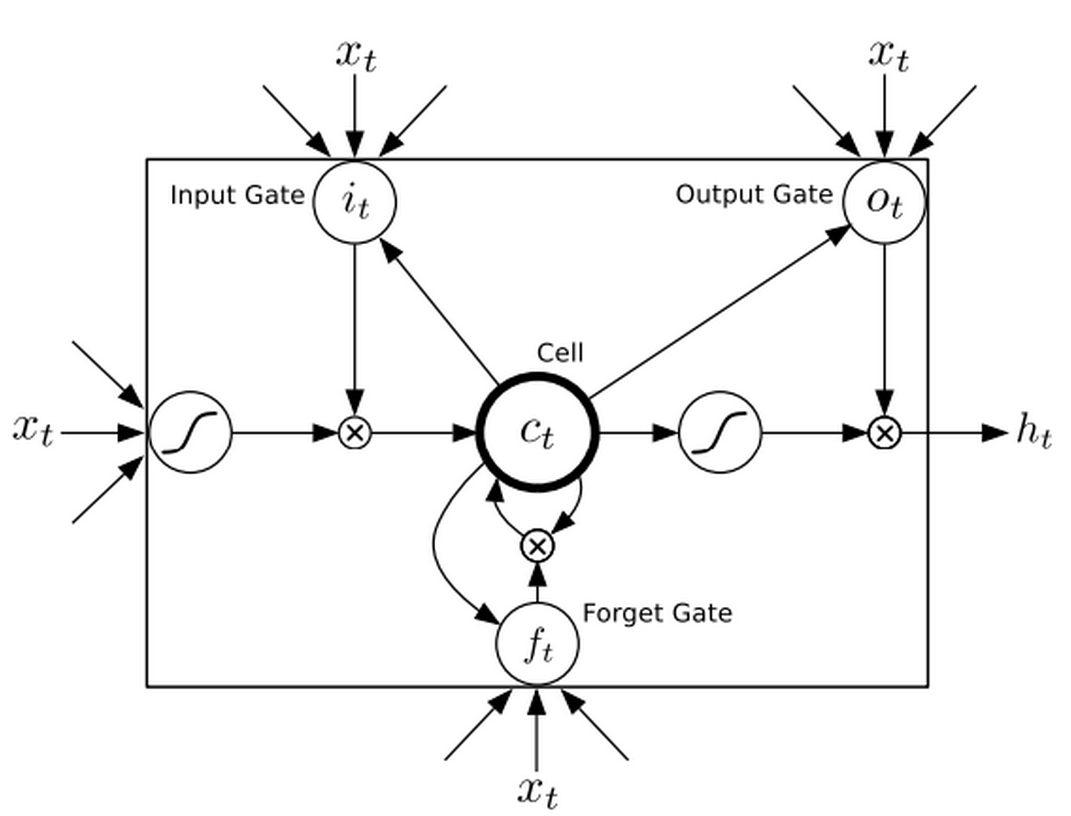
\includegraphics[width=0.8\textwidth]{lstm}
  \caption{This figure shows the basic strucuture of LSTM. In the middel, there is the memory cell which keeps the information of the data sequence. Around it, there are three gates, namely input gate, output gate and foget gate. Each of them gets information from the input and controls the updatting rule of memory cell. At the left side, there is input connection. On right side, there is output connection of this layer.}\label{series_prediction_rnn}
\end{figure}

The idea of LSTM is relatively straight forward. The memory cell stores information of the sequential data and gates in this layer tries to when and how much this information should be updated.

The basic gradient descent approach (and its backpropagation algorithm implementation) is notorious for slow convergence, because the learning rate $\gamma$ must be typically chosen small to avoid instability. Many speed-up techniques are described in the literature, 

\begin{itemize}
\item dynamic learning rate adaptation schemes. (complexity $O(TM)$, where T is number of epoch and M is number of connections)
\item use second-order gradient descent techniques, which exploit curvature of the gradient but have epoch complexity $O(TM^2)$. 
\item local error minimum
\item adding noise
\item by repeating the entire learning from different initial weight settings
\item using task-specific prior information to start from an already plausible set of weights
\end{itemize}


Starting from LSTM section

* more complex unit is called a *memory cell*
* there are many memory cells. We mark j'th cell as $c_j$.
* $c_j$ gets input from $net_{c_j}$, $out_j$(output gate), $in_j$(input gate).
* $in_j$'s activation at time t is denoted as $y^{in_j}(t)$ and we denote $out_j$'s activation at time t is denoted as $y^{out_j}(t)$

\begin{equation}
g^{out_j}(t) = f_{out_j}(net_{out_j}(t))
\end{equation}


where $f_{out_j}(\cdot (t))$ means activation function of out gate of memory cell $c_j$.

similarly:


\begin{equation}
g^{in_j}(t) = f_{in_j}(net_{int_j}(t))
\end{equation}


where $f_{in_j}(\cdot (t))$ means activation function of out gate of memory cell $c_j$.

and


\begin{equation}
net_{out_j}(t) = \sum_u w_{out_ju}y^u(t-1) \label{eq_netout}
\end{equation}


and


\begin{equation}
net_{in_j}(t) = \sum_u w_{in_ju}y^u(t-1) \label{eq_netin}
\end{equation}


We also have 


\begin{equation}
net_{c_j}(t) = \sum_u w_{c_ju}y^u(t-1) \label{eq_cell}
\end{equation}


In above $Equation~\ref{eq_netout}$, $equation~\ref{eq_netin}$, $equation~\ref{eq_cell}$, $w_{j}$ means the weight of connection from $j$'th node to $c_j$

As a consequence, the $w_{out_ju}$ means for the outgate of $j'th$ memory cell, the wight of $u'th$ connection conneted to memory cell $c_j$ and it is similar to all of the connections.

* All these dierent types of units may convey useful information about the current state of the net.
* an input gate (output gate) may use inputs from other memory cells to decide whether to store(access) certain information in its memory cell.
* There even may be recurrent self-connections like $w_{c_jc_j}$.

We have considered three conponents of memory cell. Now we consider the output of the memory cell.
The output of $c_j$ is defined as:


\begin{equation}
y^{c_j}(t) = y^{out_j}(t)h(s_{c_j}(t)) \label{eq_cell_out}
\end{equation}


Where $y^{c_j}(t)$ is the output of memory cell $c_j$ at time $t$. $y^{out_j}(t)$ is the output of outgate at time $t$. $h$ is a sigmoid function that scales the state of self-connected node which is center component of cell memory(we also call it as inner state of memory cell).

The inner state of memory cell $c_j$ is defined as:


\begin{equation}
s_{c_j}(t) = s_{c_j}(t-1) + g(t-1)\cdot y^{in_j}(t-1)
\end{equation}


Where $g(t-1) = g(net_{cj}(t))$, $g(\cdot)$ is the activation function of new input. 

* memory cell $c_j$ (the box) and its gate units $in_j$, $out_j$ builds *constant error carrousel*.(CEC)
* Distributed output representations typically do require output gates. Not always are both gate types necessary, though one may be sucient. For instance, in Experiments 2a and 2b inSection 5, it will be possible to use input gates only.
* outputgates can be benecial: they prevent the net's attempts at storing long time lag memories 


Following is the picture of the structure of the system. 

\subsection{Optimization Methods}

\section{Improved Model-Building with RNN} 
\subsection{Handling Data Noise} 
\subsection{Handling the Uncertainty of the Initial State}
\subsection{Optimal Weight Initialisation}

\chapter{Prior Arts of Combining RNN and RL}
\section{Neural Actor-Critic(idasi's group)}
\section{LSTM with POMDP objective function}
\section{PhD thesis, by Remi Coulom ?}

\section{DQN?}
\section{Hybrid Approch(RL with RNN)}
\section{Recurrent Models of Visual Attention?}       
\section{stanley gecco021 2002?}
\chapter{Experiment}
\section{RNN(LSTM) Implementation}
\section{Cart-pole Balancing Simulator}
\section{Learning a task of stacking wooden blocks}

This is a sample sentence that should look like normal text, and this
is another. This is a sample sentence that should look like normal
text, and this is another. This is a sample sentence that should look
like normal text, and this is another.


\begin{theorem}
This is a sample sentence that should look like normal text,
and this is another:
\[ y = x+3 \]
\end{theorem}

\begin{proof}
This is a sample sentence.
\end{proof}

\bibliography{library}
\bibliographystyle{siam}

\end{document}
